\documentclass[10pt]{report}

\usepackage{subcaption} % for subfigures
\usepackage{amsthm} % for QED
%\usepackage{algpseudocode} % for pseudo-code
\usepackage{mathtools} % for delimiter

\usepackage{listings} % for code
\lstset
{
	language=Matlab,
	frame=single,
	basicstyle=\footnotesize,
	captionpos=b,
	numbers=left,
	stepnumber=1,
	showstringspaces=false,
	tabsize=4,
	breaklines=true,
	breakatwhitespace=false,
}

\usepackage{siunitx} % for scientific notation
% for `e' in scientific notation
\sisetup{output-exponent-marker=\ensuremath{\mathrm{e}}}

\usepackage{float} % for figure [H]
\usepackage{booktabs} % for tabular
\usepackage{caption} % for \caption*
\usepackage[export]{adjustbox} % for valign=t
\usepackage{array} % for column type m
\usepackage{verbatim}
\usepackage{graphicx}
\graphicspath{ {imgs/} }
\usepackage{fancyhdr}
\usepackage{amssymb}
\usepackage{amsmath}

%%%%%% Pagination
\setlength{\topmargin}{-.3 in}
\setlength{\oddsidemargin}{0in}
\setlength{\evensidemargin}{0in}
\setlength{\textheight}{9.in}
\setlength{\textwidth}{6.5in}

%Title page
\newcommand{\hwTitle}{Homework \#1}
\newcommand{\hwCourse}{Numerical Differential Equations/Computational Mathematics II}
\newcommand{\hmwkClassInstructor}{Professor Shuwang Li}

\title{
	\vspace{2in}
	\textmd{\textbf{\hwCourse\\\hwTitle}}\\
	\vspace{0.3in}\large{\textit{\hmwkClassInstructor}}
	\vspace{3in}
}

%\title{Homework 1}
\author{\textbf{Zhihao Ai}}
\date{}

%Header setting. 
\pagestyle{fancy}
\fancyhead[L]{Zhihao Ai}
\fancyhead[C]{Math 478}
\fancyhead[R]{Homework 1}
%%%%%%

%Global setting.
\everymath{\displaystyle}
\setlength\parindent{0pt}

%Custom general commands.
\newcommand{\ds}{\displaystyle}
\newcommand{\f}[1] {f\left(#1\right)}
\newcommand{\eva}[2] {\left. #1 \right|_{#2}}
\newcommand{\dintt}[4] {\int_{#1}^{#2} #3 d#4}

\newcolumntype{M}[1]{>{\centering\arraybackslash}m{#1}}
\newcolumntype{C}{M{3em}}
\newcolumntype{D}{M{5em}}

\DeclarePairedDelimiter{\paren}{(}{)}
\newcommand{\abs}[1] {\left| #1 \right|}

%Custom local commands
\newcommand{\varQa} {\sqrt{\frac{3}{5}}}

\begin{document}

\maketitle

\section*{Question 1.}
\begin{enumerate}
	\item 
	(Section 6.1 Problem 23)\\
	Consider the data
	\\
	\[
		\begin{tabular}{l M{5em} M{2em} M{5em}} 
			\toprule
			$x$ & $-\sqrt{\frac{3}{5}}$ & $0$ & $\sqrt{\frac{3}{5}}$ \\ \addlinespace[0.4em]
			\hline \addlinespace[0.4em]
			$f(x)$ & $\f{-\sqrt{\frac{3}{5}}}$ & $f(0)$ & $\f{\sqrt{\frac{3}{5}}}$ \\
			\bottomrule
		\end{tabular}
	\]
	\\
	What are the Newton interpolation polynomial and the Lagrange interpolation polynomial for these data?
	
	Newton:
	\[
	c_k = \frac{y_k - p_{k-1}(x_k)}{(x_k-x_0)(x_k-x_1)\cdots(x_k-x_{k-1})}
	\]
	\begin{align*}
		c_0 &= \f{-\sqrt{\frac{3}{5}}} 
			& p_0(x)
			&= c_0
			\\
		c_1 
			&= \frac{\f{0} - p_0(0)}{0 - \paren*{-\sqrt{\frac{3}{5}}}} 
			& p_1(x)
			&= c_0 + c_1 \paren*{x - \paren*{-\sqrt{\frac{3}{5}}}}
			\\
		c_2 
			&= \frac{\f{\sqrt{\frac{3}{5}}} - p_1\paren*{\sqrt{\frac{3}{5}}}}{\paren*{\sqrt{\frac{3}{5}} - \paren*{-\sqrt{\frac{3}{5}}}} \paren*{\sqrt{\frac{3}{5}} - 0}} 
			& p_2(x)
			&= c_0 + c_1\paren*{x-\paren*{-\sqrt{\frac{3}{5}}}} + c_2\paren*{x-\paren*{-\sqrt{\frac{3}{5}}}} \paren*{x-0}
	\end{align*}
	
	Lagrange:
	\[
	l_i(x) = \prod_{\substack{j=0 \\ j\ne i}}^{n} \frac{x - x_j}{x_i - x_j}
	\]
	\begin{multline*}
	p_2(x) = \sum_{i=0}^{n} y_i l_i(x)
		= \f{-\sqrt{\frac{3}{5}}} \cdot \frac{\paren*{x-0} \paren*{x - \sqrt{\frac{3}{5}}}}{\paren*{-\sqrt{\frac{3}{5}} - 0} \paren*{-\sqrt{\frac{3}{5}} - \sqrt{\frac{3}{5}}}}
		+ \f{0} \cdot \frac{\paren*{x - \paren*{-\sqrt{\frac{3}{5}}}} \paren*{x - \sqrt{\frac{3}{5}}}}
		 {\paren*{0 - \paren*{-\sqrt{\frac{3}{5}}}} \paren*{0 - \sqrt{\frac{3}{5}}}}
		 \\
		+ \f{\sqrt{\frac{3}{5}}} \cdot \frac{\paren*{x - \paren*{-\sqrt{\frac{3}{5}}}} \paren*{x-0}} {\paren*{\sqrt{\frac{3}{5}} - \paren*{-\sqrt{\frac{3}{5}}}} \paren*{\sqrt{\frac{3}{5}} - 0}}
	\end{multline*}
	
	\item 
	(Section 6.1 Problem 15)\\
	What is the final value of $v$ in the algorithm shown?
	
	$v \leftarrow c_{i-1}$\\
	\textbf{for} $j = i$ \textbf{to} $n$ \textbf{do}\\
	\hspace*{4ex} $v \leftarrow vx + c_j$\\
	\textbf{end do}
	
	What is the number of additions and substractions involved in this algorithm?
	\begin{align*}
		v &= ((((c_{i-1}x + c_i)x + c_{i+1})x + c_{i+2})x + \cdots c_{n-1})x + c_n\\
			&= c_{i-1}x^{n-i+1} + c_ix^{n-i} + \cdots + c_{n-1}x + c_n
	\end{align*}
	The number of additions is $n-i+1$; no substractions are involved.
	
	\item 
	(Section 6.1 Problem 16)\\
	Write an efficient algorithm for evaluating
	\[
	u = \sum_{i=1}^{n} \prod_{j=1}^{i} d_j
	\]
	$u \leftarrow d_{n}$\\
	\textbf{for} $i = n-1$ \textbf{to} $1$ \textbf{step} $-1$ \textbf{do}\\
	\hspace*{4ex} $u \leftarrow d_i*(1+u)$\\
	\textbf{end do}
\end{enumerate}

\section*{Question 2.}
(Section 6.1 Problem 13)\\
Prove that if we take \textit{any} set of 23 nodes in the interval $[-1, 1]$ and interpolate the function $f(x) = \cosh{x}$ with a polynomial $p$ of degree 22, then the relative error $\abs{p(x)-f(x)}/\abs{f(x)}$ is no greater than $5 \times 10^{-16}$ on $[-1, 1]$.

Denote the nodes as $x_i, i=0,1,\cdots,22$. According to Theorem 2,
\[
f(x) - p(x) = \frac{1}{(n+1)!} \cdot f^{(n+1)}(\xi_x) \cdot \prod_{i=0}^{n} (x-x_i)
	= \frac{1}{23!} \cdot f^{(23)}(\xi_x) \cdot \prod_{i=0}^{22} (x-x_i)
\]
Since $f^{(23)}(\xi_x) = \sinh{\xi_x}$, which increases monotonically,
\[
f^{(23)}(\xi_x) < \sinh{1},\ \xi_x\in [-1, 1]
\]
Since $x\in [-1, 1]$,
\[
\prod_{i=0}^{22} (x-x_i) \le \prod_{i=0}^{22} 2 = 2^{23}
\]
Since $\cosh{x} \ge 1, f(x)\ge 1$. Therefore,
\[
\frac{\abs{p(x)-f(x)}}{\abs{f(x)}} < \frac{\frac{1}{23!} \cdot \sinh{1} \cdot 2^{23}}{1}
	\approx 3.81336\times 10^{-16}
	< 5 \times 10^{-16}
\]
\qed

\section*{Question 3.}
(Section 6.2 Problem 24)\\
Write the Newton interpolating polynomial for these data:
%\\
\[
	\begin{tabular}{lcccc} 
		\toprule
		x & 4 & 2 & 0 & 3 \\ \midrule
		f(x) & 63 & 11 & 7 & 28 \\
		\bottomrule
	\end{tabular}
\]
\\
By Theorem 1,
\[	
f[x_0, x_1, \cdots, x_n] = \frac{f[x_1, x_2, \cdots, x_n] - f[x_0, x_1, \cdots, x_{n-1}]}{x_n - x_0}
\]
we get the divided differences table:
\[
\begin{array}{cc|ccc}
4 & 63 & 26 & 6 & 1 \\
2 & 11  & 2   & 5 \\
0 & 7   & 7 \\
3 & 28
\end{array}
\]
Therefore the Newton polynomial is
\[
p(x) = 63 + 26(x-4) + 6(x-4)(x-2) + (x-4)(x-2)x
\]

\section*{Question 4.}
\begin{enumerate}
	\item 
	(Section 6.4 Problem 14)\\
	Determine whether this function is a natural cubic spline:
	\[
	f(x) = 
	\begin{cases}
		1+x-x^3, &x\in [0,1]\\
		1-2(x-1)-3(x-1)^2+4(x-1)^3, &x\in [1,2]\\
		4(x-2)+9(x-2)^2-3(x-2)^3, &x\in [2,3]\\
	\end{cases}
	\]
	By inspection, the order of $f(x)$ is no greater than 3.\\
	The first derivative of $f(x)$ is continuous:
	\[
	f'(x) = 
	\begin{cases}
	1-3x^2, &x\in [0,1]\\
	-2-6(x-1)+12(x-1)^2, &x\in [1,2]\\
	4+18(x-2)-9(x-2)^2, &x\in [2,3]\\
	\end{cases}
	\]
	The second derivative of $f(x)$ is also continuous:
	\[
	f''(x) = 
	\begin{cases}
	-6x, &x\in [0,1]\\
	-6+24x, &x\in [1,2]\\
	18-18(x-2), &x\in [2,3]\\
	\end{cases}
	\]
	Define $S_i(x),\ i=0,1,2$ as the sub-functions of $f(x)$ on $[0,1], [1,2], [2,3]$, respectively.
	\begin{align*}
		S_0(1) &= 1 = S_1(1) & S_1(2) &= 0 =S_2(2)\\
		S_0'(1) &= -1 = S_1'(1) & S_1'(2) &= 4 =S_2'(2)\\
		S_0''(1) &= -6 = S_1''(1) & S_1''(2) &= 18 =S_2''(2)
	\end{align*}
	Also we have
	\[
	f''(0) = f''(3) = 0
	\]
	Therefore, this function is a natural cubic spline.
	
	\item 
	(Section 6.4 Problem 20)\\
	Determine whether the coefficients $a, b, c,$ and $d$ exist so that the function
	\[
	S(x) = 
	\begin{cases}
	1-2x, &x\in (-\infty,-3]\\
	a+bx+cx^2+dx^3, &x\in [-3,4]\\
	157-32x, &x\in [4,+\infty)\\
	\end{cases}
	\]
	is a natural cubic spline for the interval $[-3, 4]$.
	
	Take the first and second derivatives of $S(x)$ and we have
	\[
	S'(x) = 
	\begin{cases}
	-2, &x\in (-\infty,-3]\\
	b+2cx+3dx^2, &x\in [-3,4]\\
	-32, &x\in [4,+\infty)\\
	\end{cases}
	,\ 
	S''(x) = 
	\begin{cases}
	0, &x\in (-\infty,-3]\\
	2c+6dx, &x\in [-3,4]\\
	0, &x\in [4,+\infty)\\
	\end{cases}
	\]
	For $S(x)$ to be a natural cubic spline, we need to satisfy
	\[
	\begin{cases}
	S_0(-3) = S_1(-3)\\
	S_0'(-3) = S_1'(-3)\\
	S_0''(-3) = S_1''(-3)\\
	S_1(4) = S_2(4)\\
	S_1'(4) = S_2'(4)\\
	S_1''(4) = S_2''(4)
	\end{cases}
	\Rightarrow
	\begin{cases}
	7 = a - 3 b + 9 c - 27 d\\
	-2 = b - 6 c + 27 d\\
	0 = 2 c - 18 d\\
	a + 4 b + 16 c + 64 d = 29\\
	b + 8 c + 48 d = -32\\
	2 c + 24 d = 0
	\end{cases}
	\]
	This system has no solution, as shown below:
	\[
	\left(
	\begin{array}{@{}cccc|c@{}}
		1& -3& 9& -27& 7\\
		0& 1& -6& 27& -2\\
		0& 0& 2& -18& 0\\
		1& 4& 16& 64& 29\\
		0& 1& 8& 48& -32\\
		0& 0& 2& 24& 0
	\end{array}
	\right)
	\xRightarrow{\text{R.R.}}
	\left(
	\begin{array}{@{}cccc|c@{}}
	1& 0& 0& 0& 0\\
	0& 1& 0& 0& 0\\
	0& 0& 1& 0& 0\\
	0& 0& 0& 1& 0\\
	0& 0& 0& 0& 1\\
	0& 0& 0& 0& 0
	\end{array}
	\right)
	\]
	Therefore, such $a,b,c,$ and $d$ do not exist.
\end{enumerate}

\section*{Question 5.}
(Section 6.1 Problem 37)\\
The first U.S. postage stamp was issued in 1885, with the cost to mail a letter set at 2 cents. In 1917, the cost was raised to 3 cents but then was returned to 2 cents in 1919. In 1932, it was upped to 3 cents again, where it remained for 26 years. Then a series of increases took place as follows: 1958 = 4 cents, 1963 = 5 cents, 1968 = 6 cents, 1971 = 8 cents, 1974 = 10 cents, 1978 = 15 cents, 1981 = 18 cents in March and 20 cents in October, 1985 = 22 cents, 1988 = 25 cents, 1991 = 29 cents, 1995 = 32 cents, 1999 = 33 cents, and 2001 = 34 cents. Determine the Newton interpolation polynomial for these data. Based on this, when will it cost \$1 to mail a letter? When will it cost \$10?

The following code is for calculating the coefficients and each $p(x)$:
\lstinputlisting[caption={Coefficients}]{coefficients.m}
\lstinputlisting[caption={Newton interpolation polynomial}]{newtonPoly.m}
The code below is for displaying coefficients and years when it will cost \$1 and \$10.
\lstinputlisting[caption={Find the year}]{q5p37stamp.m}

It produces the coefficent vector 
\begin{multline*}
d=[2,
0.03125,
-0.015625,
1.15077741e-03,
-2.89440714e-05,
6.78486768e-07,
-1.52159492e-08,\\
8.18727496e-10,
-9.10167759e-11,
9.40668614e-12,
-9.18167360e-13,
1.69879421e-13,\\
-2.96877259e-14,
3.92879060e-15,
-3.91394609e-16,
2.83733707e-17,
-1.60579668e-18,\\
8.19150612e-20]
\end{multline*}
Therefore, the Newton interpolation polynomial is
\begin{multline*}
	p(x) = 2 + 0.03125(x-1885) - 0.015625(x-1885)(x-1917) + \cdots +
	\\ 8.19150612e-20(x-1885)(x-1917)\cdots(x-1999)(x-2001)
\end{multline*}
By this interpolation polynomial, it costs \$1 to mail a letter in 2001.030137, which is in January, 2001; it cost \$10 in 2001.309589, which is in April, 2001.

\section*{Computer Assignment}
(Section 6.1 Problem 36)\\
The function $1/(1+x^2)$ and $e^{-x^2}$ have a similar appearance. Do they behave similarly in the interpolation process for equally spaced nodes?\\
Use the Newton interpolating polynomial $p_n(x)$ with $n=5,10,15$ on $[-5, 5]$. In each case, compute the error $f(x) - p_n(x)$ for $N = 30$ equally spaced points on $[-5, 5]$. Comment on what you get.
\lstinputlisting[caption={Interpolation on {$[-5,5]$}}]{interp.m}
\lstinputlisting[caption={Plotting functions and calculating errors}]{runge.m}
Denote $1/(1+x^2)$ as $f_a(x)$ and $e^{-x^2}$ as $f_b(x)$. The code above produces the following plots:
\begin{figure}[H]
	\centering
	\begin{subfigure}{.5\textwidth}
		\centering
		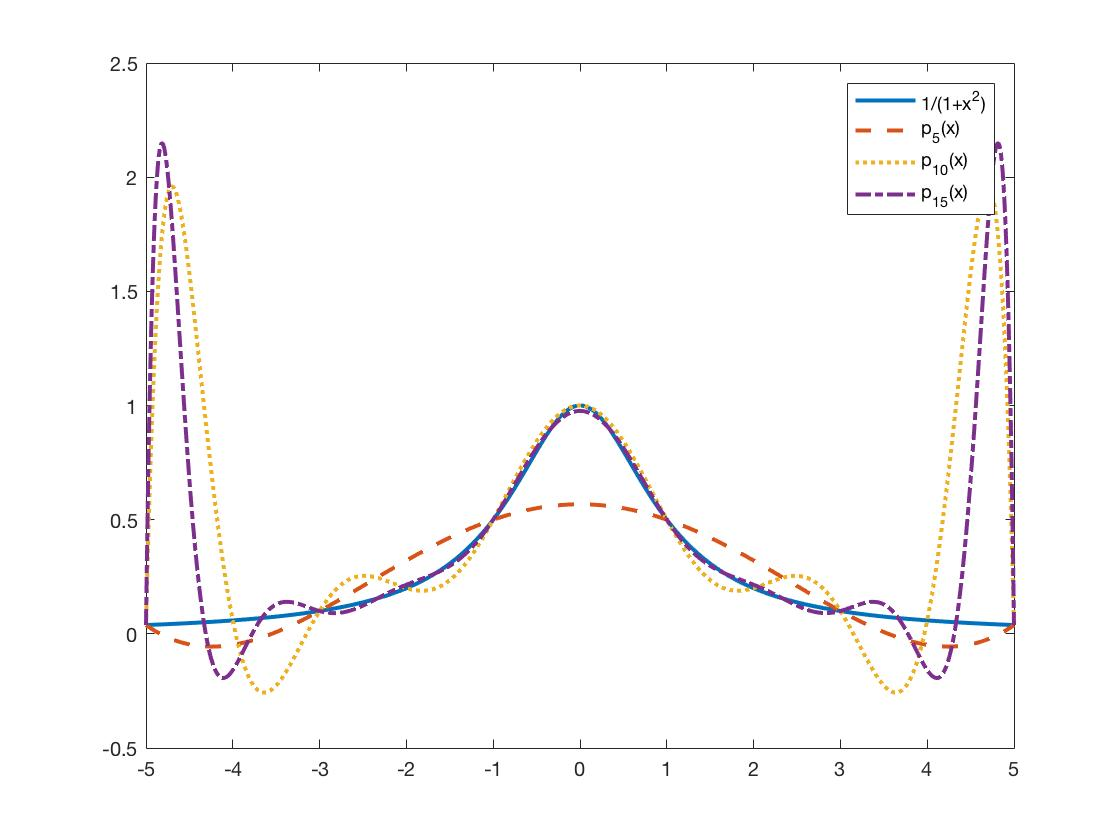
\includegraphics[width=\linewidth]{functiona.jpg}
		\caption*{$f_a(x)$ and its polynomial interpolations}
	\end{subfigure}%
	\begin{subfigure}{.5\textwidth}
		\centering
		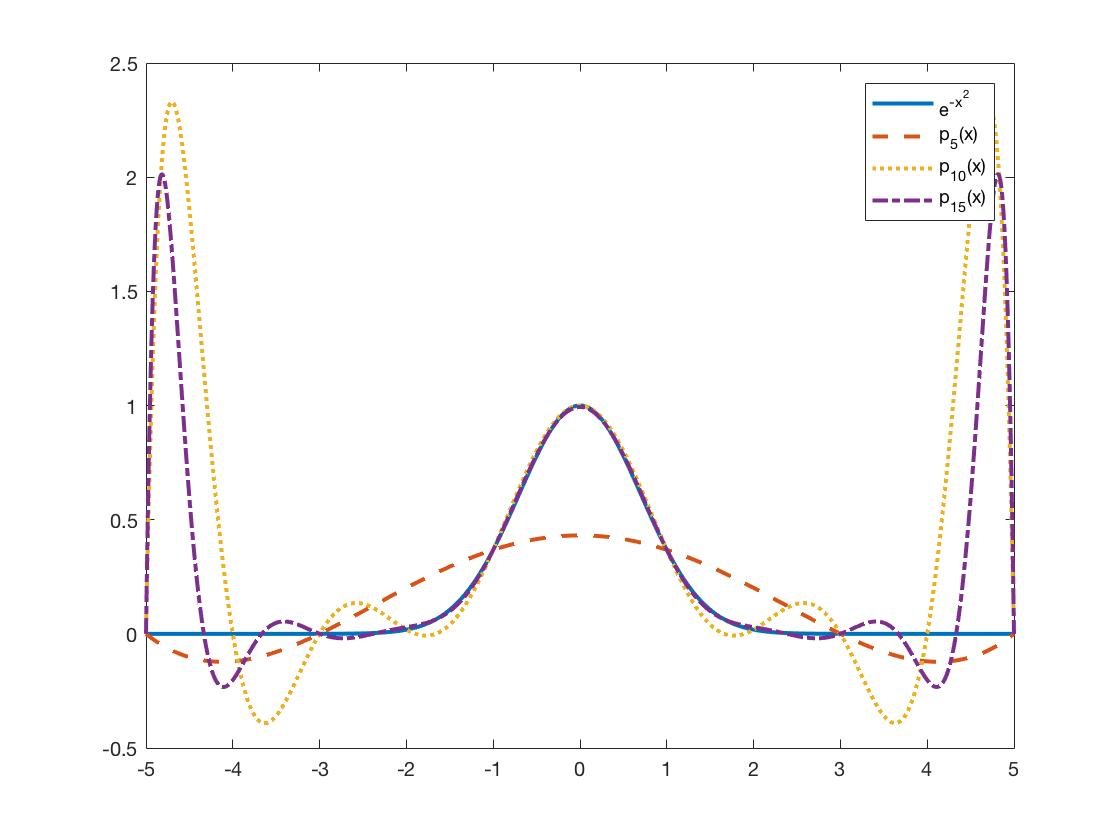
\includegraphics[width=\linewidth]{functionb.jpg}
		\caption*{$f_b(x)$ and its polynomial interpolations}
	\end{subfigure}%
\end{figure}
The errors for $N = 30$ equally spaced points on $[-5, 5]$ are:
\begin{align*}
	f_a(x) - p_{5}(x) &= 1.257120 & f_b(x) - p_{5}(x) &= 1.416331\\
	f_a(x) - p_{10}(x) &= -4.711533 & f_b(x) - p_{10}(x) &= -5.689687\\
	f_a(x) - p_{15}(x) &= -2.607657 & f_b(x) - p_{15}(x) &= -2.487981
\end{align*}
The interpolation process for equally spaced nodes for function $1/(1+x^2)$ and $e^{-x^2}$ behave similarly. For each function, the interpolating polynomial of degree 5 does not fit the curve well at the center, but on the other hand it is relatively close to the curve at the edges. In contrast, even though the polynomials of higher degree like $p_{10}(x)$ and $p_{15}(x)$ fit the curve nicely around the center, they oscillate dramatically at the edges of the interval, leading to errors even greater than the polynomial of degree 5. The comparison clearly demostrates Runge's phenomenon, which means using polynomials of high degree for interpolation can introduce much error.

\end{document}


